\makeatletter % Use \makeatletter to make '@' a letter
\def\input@path{{../}} % Define input path to parent directory
\makeatother % Restore default category code of '@'

\documentclass[../main.tex]{subfiles}

\begin{document}

\chapter{Introduction}\label{ch:introduction}

In this thesis, we focus on a specific aspect of theoretical high-energy physics and collider physics: the resummation of QCD large logarithms for 
the Thrust event-shape distribution in electron-positron ($e^+e^-$) collisions.

High energy physics, often synonymous of particle physics, and collider physics are crucial because 
they explores the most basic constituents of matter and helps us understand three of the four fundamental forces of nature: 
the strong, weak, and electromagnetic forces. Collider experiments test the predictions of the Standard Model of particle physics,
the most successful theory of particle and interactions to date. Through high precision theoretical prediction and experimental measurements,
it is possible to test the limits of the Standard Model, search for new physics beyond it and gain a better understanding of the fundamental forces. 

One key parameter of the Standard Model is the strong coupling constant $\alpha_s$, which measures the strength of the strong force.
Precise measurements of $\alpha_s$ is crucial for accurate predictions in Quantum Chromodynamics (QCD), the theory of the strong force, as all calculations in QCD
depends on it.

\begin{figure}[h!]
    \centering
    \begin{tikzpicture}
    \begin{feynman}
        \vertex (a);
        \vertex [above left=of a] (i1) {$e^{-}$};
        \vertex [below left=of a] (i2) {$e^{+}$};
        \vertex (b) [right=of a];
        \vertex [above right=of b] (f1) {$q$};
        \vertex [below right=of b] (f2) {$\bar{q}$};

        \diagram* {
            (i1) -- [fermion] (a) -- [fermion] (i2),
            (a) -- [photon, edge label=\(\gamma^*\), momentum'=\(k\)] (b),
            (f2) -- [fermion] (b) -- [fermion] (f1),
        };

    \end{feynman}
\end{tikzpicture}
    \caption{Tree-level Feynman diagram of electron-positron annihilation producing a virtual photon that decays into a quark-antiquark pair.}
    \label{fig:ep_annihilation}
\end{figure}

One example of a process studied in high-energy physics is electron-positron annihilation, as shown in \cref{fig:ep_annihilation}. 
Electron-positron annihilation has been extensively studied, particularly during the operation of the Large Electron-Positron Collider (LEP) at CERN from 1989 to 2000. 
LEP provided an optimal environment for precision studies in high-energy physics. 
Unlike hadron colliders, which are complicated by strongly interacting initial states, LEP enabled extremely accurate measurements of Standard Model quantities such as the Z-boson mass. 
These results tightly constrain beyond-the-Standard Model physics. Precision data from LEP is also used in Quantum Chromodynamics (QCD) studies, for example, to determine the strong coupling constant, $\alpha_S$.

When high-energy particles collide, quarks and gluons are produced in the interactions. Due to a phenomenon called color confinement, 
these quarks and gluons cannot exist freely and thus hadronize, forming jets of particles. A jet is a collimated stream of hadrons (such as protons, pions, and kaons)
that originates from the hadronization of a single quark or gluon.

In electron-positron annihilation, the electron and positron interact electromagnetically \\
through the exchange of a virtual photon, which mediates the electromagnetic interaction, virtual refers 
to the fact that the photon is off-shell, meaning it does not satisfy the mass-shell condition $E = pc$ for a real photon with mass $m=0$. 
This virtual photon can then decay into a quark-antiquark pair in another electromagnetic process, conserving the electrical and color charge of the initial state, as well as the four-momentum.

The quark-antiquark pair produced interacts through both the strong force and the electromagnetic force, as they possess both electric charge and color charge.
They can radiate gluons via the strong force and photons via the electromagnetic force. This radiation process continues, creating a cascade of particles known as a parton shower.
The parton shower eventually hadronizes into jets when the particles are no longer energetic enough to radiate further, and the final state particles can be revealed by the detectors, with their momenta measured to study the underlying processes.


As is typical in physics, the equations governing these interactions are highly complex so that finding exact solutions is nearly impossible.
Therefore, functions of interest are often expanded perturbatively, meaning they are expressed as a power series in a small parameter.

For the electromagnetic interaction, this small parameter is the fine structure constant (or electromagnetic coupling constant) $\alpha_{em} \sim \frac{1}{137}$.

For interactions involving the strong force, it is natural to use the aformentioned strong coupling constant, $\alpha_s$. This key parameter becomes small 
at high energies (or equivalently, short distances) due to the phenomen known as asymptotic freedom of QCD.

Extraction of $\alpha_s$ can be achieved from comparing precise QCD distribution such as the thrust event shape variable against experimental data. 


\section{Thrust variable}\label{sec:Thrust}

Thrust $T$ is defined as:

\begin{equation} \label{eq:Thrust}
    T = \max_{\vec{n}} \frac{\sum_i |\vec{p}_i \cdot \vec{n}|}{\sum_i |\vec{p}_i|} \stackrel{\text{def}}{=} 1-\tau
\end{equation}

where the sum is over all final state particles and $\vec{n}$ is a unit vector that points in the direction
which maximizes the magnitude of $T$. A quick way to calculate the thrust axis $\vec{n}$ for small number $N$ of partons in the final state is described 
in the Appendix A of \cite{Weinzierl_2009}, where the optimization problem of finding the unit vector which maximizes a certain configuration of final state partons 
is reduced to a simple loop over $2^{N-1}-1$ configurations of signs $\{s_1,\dots,s_N\}$ which satisfies the constraint
$ \vec{p}_j\cdot \vec{n} = s_j \vert \vec{p}_j\cdot \vec{n} \vert $ where $\vec{p}_j$ is the momenta of the $j$-th parton.

In practice, the sum may be carried over the detected particles only.  
The thrust distribution represents the probability of observing a given value of $T$ in $e^+e^-$ annihilation, \emph{i.e} the probability of observing a given configuration of momenta of final-state particles 
with respect to the thrust axis.

It can be seen from this definition that the thrust is an infrared and collinear safe quantity, that is, it is insensitive to the emission of zero momentum particles and to the splitting of 
one particle into two collinear ones.

In fact, contribution from soft particles with $\vec{p_i}\to 0$ drop out, and collinear splitting of a parton with 
momenta $\vec{p}$ into two partons of momenta $(1-\lambda)\vec{p}$ and $\lambda \vec{p}$ does not change the thrust:
\begin{flalign*}
    &\vert (1-\lambda)\vec{p_i}\cdot \vec{n} \vert + \vert \lambda \vec{p_i}\cdot \vec{n}\vert =(1-\lambda)\vert\vec{p_i}\cdot \vec{n} \vert + \lambda \vert \vec{p_i}\cdot \vec{n}\vert = \vert \vec{p_i}\cdot \vec{n} \vert ,\\
    &\vert (1-\lambda)\vec{p_i} \vert + \vert \lambda \vec{p_i}\vert = (1-\lambda) \vert \vec{p_i} \vert + \lambda \vert\vec{p_i}\vert = \vert \vec{p_i} \vert .
\end{flalign*}

Formally, infrared-safe observables are the one which do not distinguish between (n+1)-partons and n-partons in the soft/collinear limit, \emph{i.e},
are insensitive to what happens at long-distance (non-perturbative) scales.

Infrared safe observables are important in the context of perturbative QCD, because they allow for a meaningful comparison between theory and experiment. 

A significant challenge in achieving precise theoretical predictions from QCD lies in the complexity of the relevant fixed-order calculations. While the next-to-leading-order (NLO) results 
for event shapes have been known since 1980 \cite{Ellis:1980wv}, the relevant next-to-next-leading order (NNLO) calculations were completed only in 2007 \cite{Gehrmann-DeRidder:2007nzq}.

\begin{figure}[h]
    \centering
    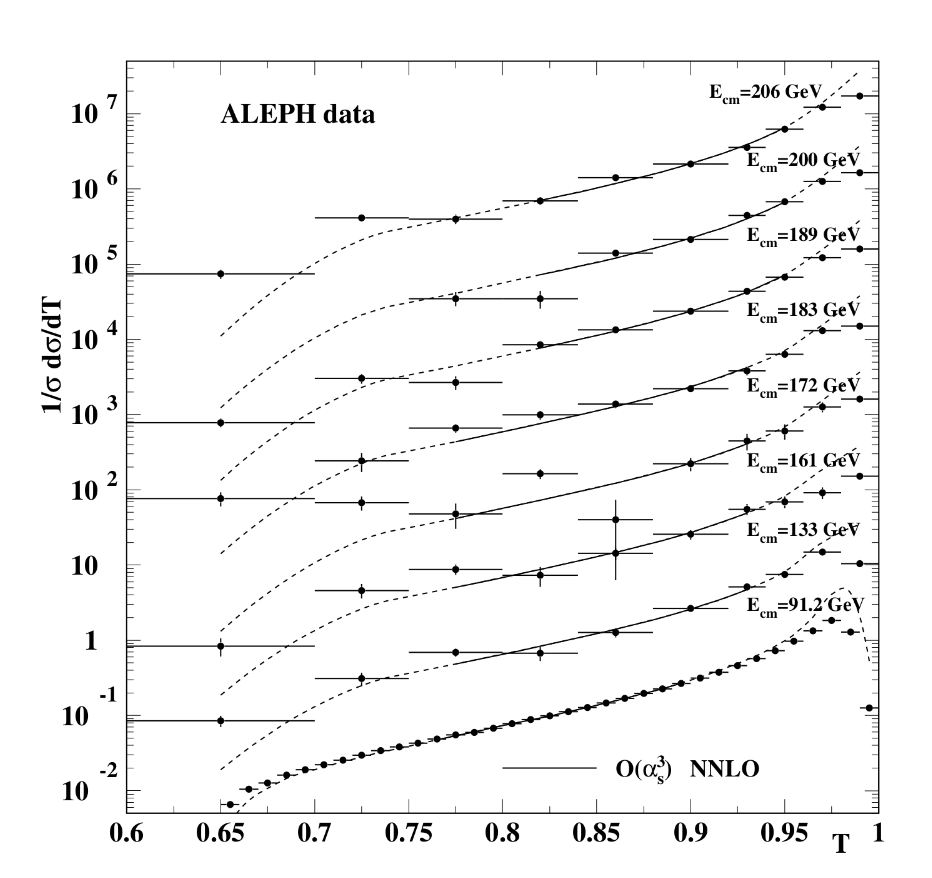
\includegraphics[width=0.5\textwidth]{figures/LEP_Thrust_NNLO.png}
    \caption{Distributions measured by ALEPH, after correction for backgrounds and detector
    effects of thrust at energies between 91.2 and 206
    GeV together with NNLO QCD predictions. The error bars correspond to statistical
    uncertainties. The plotted
    distributions are scaled by arbitrary factors for presentation. Image taken from \cite{Dissertori_2008}.}
    \label{fig:LEP_Thrust_NNLO}
\end{figure}

From \cref{fig:LEP_Thrust_NNLO},  it is evident that the NNLO prediction agrees well with the data, except in the region near $T=0.5$ (spherical final state) and $T=1$ (pencil-like final state).

This is because thrust distribution for $T\simeq 1$ is dominated by two-jet configurations, \emph{i.e.} the final state particles consist of two partons emitted back-to-back like \cref{fig:ep_annihilation}.
In contrast, the tail of the distribution near $T= 0.5$ is dominated by multijet final states.

To improve the agreement between theory and experiment, we'll need higher fixed order calculations (challenging task), but this will only 
improve the agreement in the tail region, to also improve the agreement in the dijet region we need to use resummation techniques.


\subsection{Thrust distribution} \label{subsec:Thrust_distribution}

The cross section is defined as the probability of observing a final state with a given thrust value $\tau$ and Thrust distribution is expressed in three ways:
as a differential cross section, as a cumulative distribution and as its Laplace transform.

\begin{equation}\label{eq:differential_cross_section}
    \sigma(\tau) =  \frac{1}{\sigma_0} \dv{\sigma}{\tau}
\end{equation}

\begin{equation}\label{eq:cumulative_distribution}
    R_T(\tau) = \int^\tau_0 \dd{\tau'} \frac{1}{\sigma_0}\dv{\sigma}{\tau'}
\end{equation}

\begin{equation}\label{eq:Laplace transform distribution}
    \Tilde{\sigma}(\nu) = \int^\infty_0 \dd{\tau} e^{-\nu \tau} \dv{\sigma}{\tau}
\end{equation}

It can be seen that a two-particle final state has fixed $T = 1$, in fact at the zeroth order of the fixed order this corresponds to a delta distribution 
for the differential cross section, as shown in  \cref{eq:LO fixed order}, consequently the thrust distribution receives its first non-trivial contribution 
from three-particle final states.

The lower limit on $T$ depends on the number of final-state particles.
Neglecting masses, for three particles, $T_{min} = 2/3$, corresponding to a symmetric configuration.
For four particles the minimum thrust corresponds to final-state momenta forming the vertices of a regular tetrahedron,
each making an angle $\cos^{-1}(1/\sqrt{3})$ with respect to the thrust axis. Thus $T_{min} = 1/\sqrt{3} \approx 0.577$ in this
case. For more than four particles, $T_{min}$ approaches $1/2$ from above as the number of particles increases.

At large values of $T$, however, there are terms in higher order that become enhanced by powers of $\ln(1 - T)$.
In this kinematical region the real expansion parameter is the large effective coupling $\alpha_s \ln^2(\tau)$ and therefore
any finite-order perturbative calculation cannot give an accurate evaluation of the cross section.

For example, at leading order in perturbation theory the thrust distribution has the form:

\begin{equation}\label{eq:LO fixed order}
    \frac{1}{\sigma_0}\dv{\sigma}{\tau} = \delta(\tau) + \frac{2\alpha_s}{3\pi} \qty[\frac{-4 \ln \tau - 3}{\tau} + \dots]_{+}
\end{equation}

where $\sigma_0$ is the born cross section, the ellipsis denotes terms that are regular as $\tau \to 0$ and the subscript $+$ denotes the 
plus distribution, which is defined as:

\begin{equation}
    \qty[\frac{-4 \ln \tau - 3}{\tau}]_{+} = \lim_{\epsilon \to 0}\qty[ \qty(\frac{-4 \ln \tau - 3}{\tau}) \theta(\tau - \epsilon) +\delta(\tau - \epsilon)\int_1^{\tau}  \dd{\tau'} \qty(\frac{-4 \ln \tau' - 3}{\tau'})]
\end{equation}

Upon integration over $\tau$, we obtain the cumulative distribution:

\begin{flalign}
    R_T(\tau) &= \int_0^\tau \dd{\tau'} \frac{1}{\sigma_0}\dv{\sigma}{\tau'} \nonumber \\
    &= 1 + \frac{2\alpha_s}{3\pi} + \lim_{\epsilon \to 0} \qty[ \int_\epsilon^\tau  \dd{\tau'} \qty(\frac{-4 \ln \tau' - 3}{\tau'} + \dots) + \int_1^{\epsilon}  \dd{\tau'} \qty(\frac{-4 \ln \tau' - 3}{\tau'}+\dots)]\\
    &= 1 + \frac{2\alpha_s}{3\pi} \qty[-2 \ln^2 \tau - 3 \ln \tau + \dots] \nonumber
\end{flalign}

Double logarithmic terms of the form $\alpha_s^n \ln^{2n}\tau$ plagues the fixed order expansion in the strong coupling. In the dijet region, higher order 
terms are as important as lower order ones, necessitating resummation to achieve reliable predictions.

\subsection{Fixed Order Cross Section}

The fixed-order thrust differential distribution has been calculated to leading order analytically and
to NLO and NNLO numerically, as mentioned earlier. At a centre-of-mass energy $Q$ and for a renormalization scale $\mu$ takes the form:

\begin{equation}\label{eq:Fixed_order}
    \frac{1}{\sigma_0} \dv{\sigma}{\tau} \qty(\tau,Q) = \delta(\tau) + \frac{\alpha_s(\mu)}{2\pi}\dv{A}{\tau} \qty(\tau) + \qty(\frac{\alpha_s(\mu)}{2\pi})^2 \dv{B}{\tau} \qty(\tau,\frac{\mu}{Q}) + \qty(\frac{\alpha_s(\mu)}{2\pi})^3 \dv{C}{\tau} \qty(\tau,\frac{\mu}{Q}) + \order{\alpha_s^4}
\end{equation}

where the complete leading order expression for the thrust distribution reads \cite{Ellis:1980wv}:

\begin{equation}\label{eq:Fixed_order_A}
    \dv{A}{\tau}(\tau) =  \text{C}_F \left(9 \tau -\frac{3}{\tau }+\left(-6 +\frac{4}{(1-\tau ) \tau }\right) \ln \left(\frac{1-2 \tau }{\tau }\right)+6\right)
\end{equation}

with $C_F = \frac{4}{3}$ the Casimir of the fundamental representation of SU(3). As mentioned earlier, this expansion becomes unreliable near the dijet limit $\tau \to 0$ due to the presence of large logarithms.
Resummation of these terms to all orders in $\alpha_s$ is necessary to obtain a reliable prediction.

While the cumulant distribution has the following fixed-order expansion:

\begin{equation}\label{eq:Fixed_order_R}
    R_T(\tau) = 1 + A(\tau) \frac{\alpha_s(\mu)}{2\pi} + B(\tau,\mu) \frac{\alpha_s(\mu)}{2\pi}^2 + C(\tau,\mu)\frac{\alpha_s(\mu)}{2\pi}^3 + \order{\alpha_s^4} ,
\end{equation}

the fixed-order coeficcient $A,B$ and $C$ can be obtained by integrating the differential cross section \cref{eq:Fixed_order_A} to all order and 
imposing the normalization condition $R(\tau_{max}) = 1$, where $\tau_{max}$ is the maximum kinetically allowed value of $\tau$. At leading order ($e^+e^- \to q\bar{q}g$) $\tau_{max}=\frac{1}{3}$, at Next-to-Leading Order
is $\tau_{max}=1-\frac{1}{\sqrt{3}}$ and from NNLO onwards $\tau_{max}$ needs to be estimated numerically.

At leading order we have:

\begin{flalign} \label{eq:Fixed_order_A_integrated}
    A(\tau) = \int_0^\tau \dd{\tau'} \dv{A}{\tau'}(\tau') &= C_F \Bigl(\frac{9 \tau ^2}{2}-2 \ln ^2(1-\tau )-2 \ln ^2(\tau )+6 \tau  (\ln (\tau )+1) &\nonumber \\
    &+4 \ln (1-\tau ) \ln (\tau )-3 \ln (\tau )+3 (1-2 \tau ) \ln (1-2 \tau) \\
    &-4 \text{Li}_2\left(\frac{\tau }{1-\tau }\right)\Bigr) . \nonumber
\end{flalign}

\end{document}